%%%%%%%%%%%%%%%%%%%%%%%%%%%%%%%%%%%%%%%%%
% Arsclassica Article
% LaTeX Template
% Version 1.1 (1/8/17)
%
% This template has been downloaded from:
% http://www.LaTeXTemplates.com
%
% Original author:
% Lorenzo Pantieri (http://www.lorenzopantieri.net) with extensive modifications by:
% Vel (vel@latextemplates.com)
%
% License:
% CC BY-NC-SA 3.0 (http://creativecommons.org/licenses/by-nc-sa/3.0/)
%
%%%%%%%%%%%%%%%%%%%%%%%%%%%%%%%%%%%%%%%%%

%----------------------------------------------------------------------------------------
%	PACKAGES AND OTHER DOCUMENT CONFIGURATIONS
%----------------------------------------------------------------------------------------

\documentclass[
10pt, % Main document font size
a4paper, % Paper type, use 'letterpaper' for US Letter paper
oneside, % One page layout (no page indentation)
%twoside, % Two page layout (page indentation for binding and different headers)
headinclude,footinclude, % Extra spacing for the header and footer
BCOR5mm, % Binding correction
]{scrartcl}

%%%%%%%%%%%%%%%%%%%%%%%%%%%%%%%%%%%%%%%%%
% Arsclassica Article
% Structure Specification File
%
% This file has been downloaded from:
% http://www.LaTeXTemplates.com
%
% Original author:
% Lorenzo Pantieri (http://www.lorenzopantieri.net) with extensive modifications by:
% Vel (vel@latextemplates.com)
%
% License:
% CC BY-NC-SA 3.0 (http://creativecommons.org/licenses/by-nc-sa/3.0/)
%
%%%%%%%%%%%%%%%%%%%%%%%%%%%%%%%%%%%%%%%%%

%----------------------------------------------------------------------------------------
%	REQUIRED PACKAGES
%----------------------------------------------------------------------------------------

\usepackage[
nochapters, % Turn off chapters since this is an article        
beramono, % Use the Bera Mono font for monospaced text (\texttt)
eulermath,% Use the Euler font for mathematics
pdfspacing, % Makes use of pdftex’ letter spacing capabilities via the microtype package
dottedtoc % Dotted lines leading to the page numbers in the table of contents
]{classicthesis} % The layout is based on the Classic Thesis style

\usepackage{arsclassica} % Modifies the Classic Thesis package

\usepackage[T1]{fontenc} % Use 8-bit encoding that has 256 glyphs

\usepackage[utf8]{inputenc} % Required for including letters with accents

\usepackage{graphicx} % Required for including images
\graphicspath{{Figures/}} % Set the default folder for images

\usepackage{enumitem} % Required for manipulating the whitespace between and within lists

\usepackage{lipsum} % Used for inserting dummy 'Lorem ipsum' text into the template

\usepackage{subfig} % Required for creating figures with multiple parts (subfigures)

\usepackage{amsmath,amssymb,amsthm} % For including math equations, theorems, symbols, etc

\usepackage{varioref} % More descriptive referencing

%----------------------------------------------------------------------------------------
%	THEOREM STYLES
%---------------------------------------------------------------------------------------

\theoremstyle{definition} % Define theorem styles here based on the definition style (used for definitions and examples)
\newtheorem{definition}{Definition}

\theoremstyle{plain} % Define theorem styles here based on the plain style (used for theorems, lemmas, propositions)
\newtheorem{theorem}{Theorem}

\theoremstyle{remark} % Define theorem styles here based on the remark style (used for remarks and notes)

%----------------------------------------------------------------------------------------
%	HYPERLINKS
%---------------------------------------------------------------------------------------

\hypersetup{
%draft, % Uncomment to remove all links (useful for printing in black and white)
colorlinks=true, breaklinks=true, bookmarks=true,bookmarksnumbered,
urlcolor=webbrown, linkcolor=RoyalBlue, citecolor=webgreen, % Link colors
pdftitle={}, % PDF title
pdfauthor={\textcopyright}, % PDF Author
pdfsubject={}, % PDF Subject
pdfkeywords={}, % PDF Keywords
pdfcreator={pdfLaTeX}, % PDF Creator
pdfproducer={LaTeX with hyperref and ClassicThesis} % PDF producer
} % Include the structure.tex file which specified the document structure and layout

\hyphenation{Fortran hy-phen-ation} % Specify custom hyphenation points in words with dashes where you would like hyphenation to occur, or alternatively, don't put any dashes in a word to stop hyphenation altogether

%----------------------------------------------------------------------------------------
%	TITLE AND AUTHOR(S)
%----------------------------------------------------------------------------------------

\title{\normalfont\spacedallcaps{Notes on Machine Learning}} % The article title

%\subtitle{Subtitle} % Uncomment to display a subtitle

\author{\spacedlowsmallcaps{Bruno Ximenez} }% The article author(s) - author affiliations need to be specified in the AUTHOR AFFILIATIONS block

\date{} % An optional date to appear under the author(s)

%----------------------------------------------------------------------------------------

\begin{document}

%----------------------------------------------------------------------------------------
%	HEADERS
%----------------------------------------------------------------------------------------

\renewcommand{\sectionmark}[1]{\markright{\spacedlowsmallcaps{#1}}} % The header for all pages (oneside) or for even pages (twoside)
%\renewcommand{\subsectionmark}[1]{\markright{\thesubsection~#1}} % Uncomment when using the twoside option - this modifies the header on odd pages
\lehead{\mbox{\llap{\small\thepage\kern1em\color{halfgray} \vline}\color{halfgray}\hspace{0.5em}\rightmark\hfil}} % The header style

\pagestyle{scrheadings} % Enable the headers specified in this block

%----------------------------------------------------------------------------------------
%	TABLE OF CONTENTS & LISTS OF FIGURES AND TABLES
%----------------------------------------------------------------------------------------

\maketitle % Print the title/author/date block

\setcounter{tocdepth}{2} % Set the depth of the table of contents to show sections and subsections only

\tableofcontents % Print the table of contents

\listoffigures % Print the list of figures

\listoftables % Print the list of tables

%----------------------------------------------------------------------------------------
%	ABSTRACT
%----------------------------------------------------------------------------------------

\section*{Abstract} % This section will not appear in the table of contents due to the star (\section*)

% \lipsum[1] % Dummy text

%----------------------------------------------------------------------------------------
%	AUTHOR AFFILIATIONS
%----------------------------------------------------------------------------------------

% \let\thefootnote\relax\footnotetext{* \textit{Department of Biology, University of Examples, London, United Kingdom}}

% \let\thefootnote\relax\footnotetext{\textsuperscript{1} \textit{Department of Chemistry, University of Examples, London, United Kingdom}}

%----------------------------------------------------------------------------------------

\newpage % Start the article content on the second page, remove this if you have a longer abstract that goes onto the second page

%----------------------------------------------------------------------------------------
%	INTRODUCTION
%----------------------------------------------------------------------------------------

\section{Week 1 -- Introduction}

% A statement requiring citation \cite{Figueredo:2009dg}.

% \lipsum[1-3] % Dummy text

% Some mathematics in the text: $\cos\pi=-1$ and $\alpha$.
 
%----------------------------------------------------------------------------------------
%	Weeks
%----------------------------------------------------------------------------------------

\section{Week 2 -- Linear regression}

The linear regreession consists in finding best fit parameters of a linear function that will be used as a model 
or hypothesis. The mathematical expression is:

\begin{equation} \label{h}
    h_{\theta}(x) = \theta_{0} + \theta_{1} x
\end{equation}
This is the case of a one dimensional model i.e. y is a function of one variable. In machine learning language, the variables will be called features.
It is very convinient, specially from the point of view of code implementation, to write this function in vectorial form. 
The parameters $\theta_{j}$ are written as a single column vector $\theta = (\theta_{0}, \theta_{1})$. The feature is written in the vector form by using the trick
of adding a dimension with a unit value representing $x^{0}$: $X = (x_{0}=1, x_{1})$. The hypothesis \ref{h} is then simplified:

\begin{equation}
    h_{\theta}(x) = X \cdot \theta
\end{equation}
Recalling that dim($X$) =  $m \times (n+1)$ matrix (assemble of column vectors) and $\theta$ is a column vector, dim($\theta$) = $(n+1) \times 1$,
where $m$ is the number of training examples and $n$ is the number of variables or features.
The task of the linear regression method is to, given a training data set $(x,y)$, find the best parameters $\theta$ that will fit the model to the data.
Based on this, one can use the output of the calculation to predict or to estimate $y$. The search for the optimum parameters can be done by writing the function:

\begin{equation}
    \begin{split}
        J(\theta) &= \frac{1}{2 m} \sum _{k=1}^{m} [ h_{\theta}(x^{(k)}) - y^{(k)}]^{2} \\
                    & = \frac{1}{2 m} (X \cdot \theta - y)^{T} \cdot (X \cdot \theta - y)
    \end{split}
\end{equation}
called the cost function. It is proportional to the square of the difference between the model and the trainning data set. 
The last step is to find a routine that can minimize the cost function. One way to do this is to use the gradient descendent 
method by calculating in an iterative manner the parameters using the equation:

\begin{equation} \label{grad_desc}
    \theta_{i} = \theta_{i} - \alpha \frac{\partial J}{\partial \theta}
\end{equation}
where $\alpha$, the learning rate, is a parameter to be adjusted and will control the convergence speed of the algorithm. 
Values of $\alpha$ that are too large will make the algorithm to overshoot and never reach the minimum
value while a too small $\alpha$ may slow the code down. An optimum value must be found. It is worth mentioning that the operator "="
is being used here as an assignment operator and not truth assertion.

Equation \ref{grad_desc} can be explicitly calculated:

\begin{equation}
    \begin{split}
        \theta_{i} & = \theta_{i} - \frac{\alpha}{m} \sum _{k=1}^{m} [ h_{\theta}(x^{(k)}) - y^{(k)}] x_{i}^{(k)} \\
                   \theta & = \theta - \frac{\alpha}{m} X^{T} \cdot (X \cdot \theta - y)
    \end{split}
\end{equation}

Writting the equations in the vector form allows us to calculate the updated values in a simultaneous way for all parameters,
which is the desired routine. From the coding point of view, the summation form requires the use of a iterative for loop over the 
vectors and matrices (and one needs to be carefull with ensuring the simultaneous update of the parameters) while the vector form is a simple single line of code (simultaneous by definition).

For a multi-dimensional problems i.e. with more than one feature, in the vectorial form, the problem is exact the same and no change need 
to be made in the equations. The expression for the hypothesis is modified as:

\begin{equation}
    \begin{split}
        h_{\theta}(x) & = \sum_{i=1}^{n} \theta_{i} x_{i} \\
                        & = X \cdot \theta
    \end{split}
\end{equation}
with $x_{0} = 1$.
\section{Week 3 -- Logistic regression}

We turn our attention now to the classification problem in supervised learning, which consists of classifying 
the data into a discrete number of labels. The simplest is the binary of binomial one with the data being classified as
yes or no, 0 or 1, true or false, etc. 

In this case, the linear hypothesis is not suitable anymore and it will be replaced by the sigmoid function defined as:

\begin{equation}
    g(z) = \frac{1}{1 + e^{-z}}
\end{equation}
with,
\begin{equation}
    z = X \cdot \theta
\end{equation}

Some properties of the sigmoid function:
\begin{equation}
    g(z) = 
        \begin{cases}
            0 &  z \rightarrow -\infty \\
            0.5 & z = 0 \\
            1 & z \rightarrow +\infty
        \end{cases}
\end{equation}

The interpretation is given in terms of probability: \textit{the probability of a given input produce an output = 1 is precisely}:

\begin{equation}
    P(y=1|x;\theta) = g(z)
\end{equation}
Thus , for $z \geqslant 0$ the probability of $y=1$ is equal or bigger than 0.5. The prediction or guess is a decision wether to 
label the data as 1 or 0. An educated guess is to set the boundary between the two discrete labels at $z=0$. That is called \textit{decision boundary}.


\subsection{Cost function}

Here I will describe how to write the cost function for the logistic regression.
The cost function will be modified according to the equations below. The specific choice of this model comes from statistical theory of maximum likelyhood (look for better reasoning here).

\begin{equation} \label{}
    J(\theta) = \frac{1}{m} \sum_{i=1}^{m} Cost(g(z^{(i)}), y^{(i)})
\end{equation}

With,

\begin{equation}
    Cost[g(z^{(i)}), y^{(i)}] =
        \begin{cases}
            - log[g(z^{(i)})] & \text{if  } y = 1 \\
            - log[1- g(z^{(i)})] & \text{if  }  y = 0
        \end{cases}
\end{equation}

In equation form:

\begin{equation}
    Cost[g(z^{(i)}), y^{(i)}] = - y log[g(z^{(i)})] - (1 - y)log[1- g(z^{(i)})]
\end{equation}

And,

\begin{equation}
    J(\theta) = - \frac{1}{m} \sum_{i=1}^{m} y^{(i)} log[g(z^{(i)})] + (1 - y^{(i)})log[1- g(z^{(i)})]
\end{equation}

To minimize this function, the same strategy is used:

\begin{equation}
    \theta_{i} = \theta_{i} - \alpha \frac{\partial }{\partial \theta} J(\theta)
\end{equation}

Or, in a vectorized implementation:

\begin{equation}
    \theta = \theta - \frac{\alpha}{m} X^{T} (g(X\cdot\theta) - Y)
\end{equation}




% \lipsum[5] % Dummy text

% \begin{enumerate}[noitemsep] % [noitemsep] removes whitespace between the items for a compact look
% \item First item in a list
% \item Second item in a list
% \item Third item in a list
% \end{enumerate}

%------------------------------------------------

% \subsection{Paragraphs}

% \lipsum[6] % Dummy text

% \paragraph{Paragraph Description} \lipsum[7] % Dummy text

% \paragraph{Different Paragraph Description} \lipsum[8] % Dummy text

%------------------------------------------------

% \subsection{Math}

% \lipsum[4] % Dummy text

% \begin{equation}
% \cos^3 \theta =\frac{1}{4}\cos\theta+\frac{3}{4}\cos 3\theta
% \label{eq:refname2}
% \end{equation}

% \lipsum[5] % Dummy text

% \begin{definition}[Gauss] 
% To a mathematician it is obvious that
% $\int_{-\infty}^{+\infty}
% e^{-x^2}\,dx=\sqrt{\pi}$. 
% \end{definition} 

% \begin{theorem}[Pythagoras]
% The square of the hypotenuse (the side opposite the right angle) is equal to the sum of the squares of the other two sides.
% \end{theorem}

% \begin{proof} 
% We have that $\log(1)^2 = 2\log(1)$.
% But we also have that $\log(-1)^2=\log(1)=0$.
% Then $2\log(-1)=0$, from which the proof.
% \end{proof}

% %----------------------------------------------------------------------------------------
%	RESULTS AND DISCUSSION
%----------------------------------------------------------------------------------------

% \section{Results and Discussion}

% Reference to Figure~\vref{fig:gallery}. % The \vref command specifies the location of the reference

% \begin{figure}[tb]
% \centering 
% 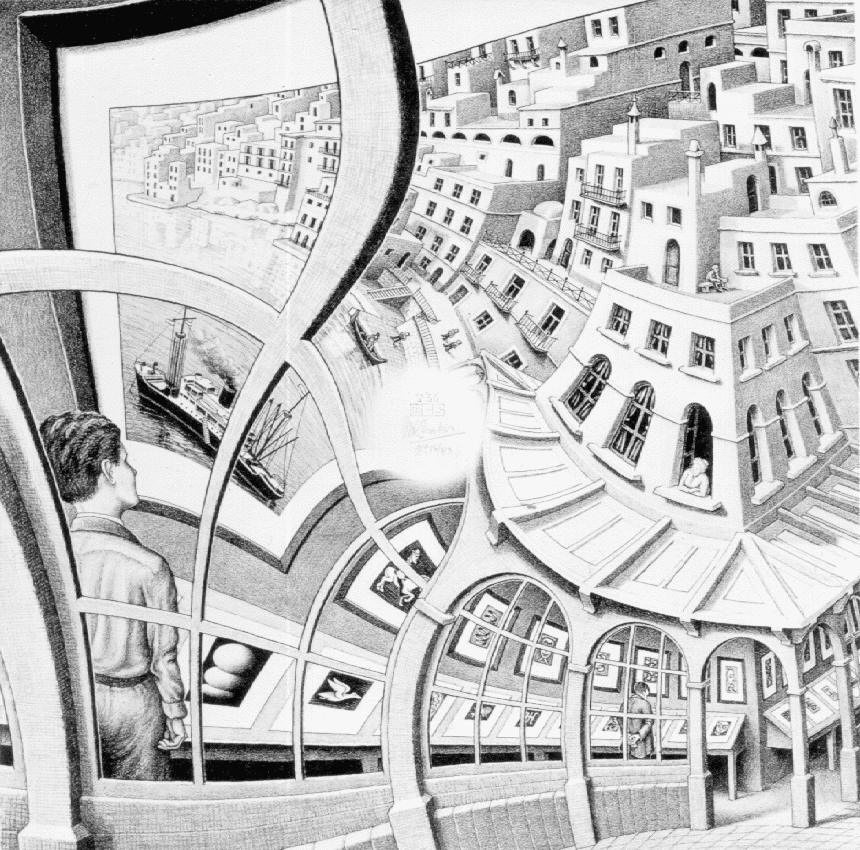
\includegraphics[width=0.5\columnwidth]{GalleriaStampe} 
% \caption[An example of a floating figure]{An example of a floating figure (a reproduction from the \emph{Gallery of prints}, M.~Escher,\index{Escher, M.~C.} from \url{http://www.mcescher.com/}).} % The text in the square bracket is the caption for the list of figures while the text in the curly brackets is the figure caption
% \label{fig:gallery} 
% \end{figure}

% \lipsum[10] % Dummy text

% %------------------------------------------------

% \subsection{Subsection}

% \lipsum[11] % Dummy text

% \subsubsection{Subsubsection}

% \lipsum[12] % Dummy text

% \begin{description}
% \item[Word] Definition
% \item[Concept] Explanation
% \item[Idea] Text
% \end{description}

% \lipsum[12] % Dummy text

% \begin{itemize}[noitemsep] % [noitemsep] removes whitespace between the items for a compact look
% \item First item in a list
% \item Second item in a list
% \item Third item in a list
% \end{itemize}

% \subsubsection{Table}

% \lipsum[13] % Dummy text

% \begin{table}[hbt]
% \caption{Table of Grades}
% \centering
% \begin{tabular}{llr}
% \toprule
% \multicolumn{2}{c}{Name} \\
% \cmidrule(r){1-2}
% First name & Last Name & Grade \\
% \midrule
% John & Doe & $7.5$ \\
% Richard & Miles & $2$ \\
% \bottomrule
% \end{tabular}
% \label{tab:label}
% \end{table}

% Reference to Table~\vref{tab:label}. % The \vref command specifies the location of the reference

%------------------------------------------------

% \subsection{Figure Composed of Subfigures}

% Reference the figure composed of multiple subfigures as Figure~\vref{fig:esempio}. Reference one of the subfigures as Figure~\vref{fig:ipsum}. % The \vref command specifies the location of the reference

% \lipsum[15-18] % Dummy text

% \begin{figure}[tb]
% \centering
% \subfloat[A city market.]{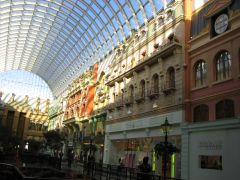
\includegraphics[width=.45\columnwidth]{Lorem}} \quad
% \subfloat[Forest landscape.]{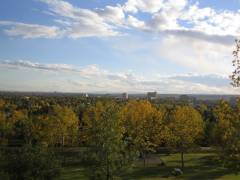
\includegraphics[width=.45\columnwidth]{Ipsum}\label{fig:ipsum}} \\
% \subfloat[Mountain landscape.]{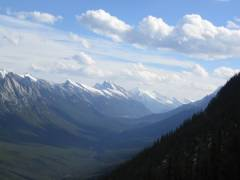
\includegraphics[width=.45\columnwidth]{Dolor}} \quad
% \subfloat[A tile decoration.]{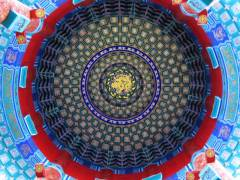
\includegraphics[width=.45\columnwidth]{Sit}}
% \caption[A number of pictures.]{A number of pictures with no common theme.} % The text in the square bracket is the caption for the list of figures while the text in the curly brackets is the figure caption
% \label{fig:esempio}
% \end{figure}

%----------------------------------------------------------------------------------------
%	BIBLIOGRAPHY
%----------------------------------------------------------------------------------------

\renewcommand{\refname}{\spacedlowsmallcaps{References}} % For modifying the bibliography heading

\bibliographystyle{unsrt}

\bibliography{sample.bib} % The file containing the bibliography

%----------------------------------------------------------------------------------------

\end{document}